\documentclass{article}
\usepackage{graphicx}
\usepackage[french]{babel}
\usepackage{multicol}
\usepackage{geometry}
\usepackage{titling}
\usepackage[utf8]{inputenc}





\geometry{
    a4paper,
    total={170mm,257mm},
    left=20mm,
    top=30mm,
}



\title{
    
\includegraphics[width=1\textwidth]{logo/titre.png} \\
    \vspace{1.5cm}
    {\Huge \textbf{Rapport phase 3}} \\
    \vspace{1.5cm}
}

\author{
    \textbf{Moussaoui Noah , Boumeddien Benkechida Houari , Camur Abdullah , Sablon Guillaume} \\
    Université catholique de Louvain-la-Neuve \\
    Campus de Charleroi, EPL en SINC 
}

\date{
    \vspace{1.5cm}
    Durée de travail : Mars 2024 - Mai 2024 \\
     \vspace{1.5cm}
    
\includegraphics[width=0.5\textwidth]{logo/EPL.jpeg}
}

\begin{document}

\begin{titlingpage}
\maketitle
\end{titlingpage}

\newpage
\tableofcontents
\newpage

\section{ Introduction }

Nous avons créé un site sur la mobilité en Belgique. Notre thème était de retourner un peu dans les sites des années 2000. Notre but était de rendre accessible les données sur la mobilité en Belgique à l'aide de graphiques et de pages de sélection tout en plongeant l'utilisateur dans une ambiance rétro avec de la musique et un jeu un peu old school de notre enfance : le mémo. Alors voici comment nous avons ressuscité les sites des années 2000 avec le codage moderne.

\section{Home page}

\begin{center}
    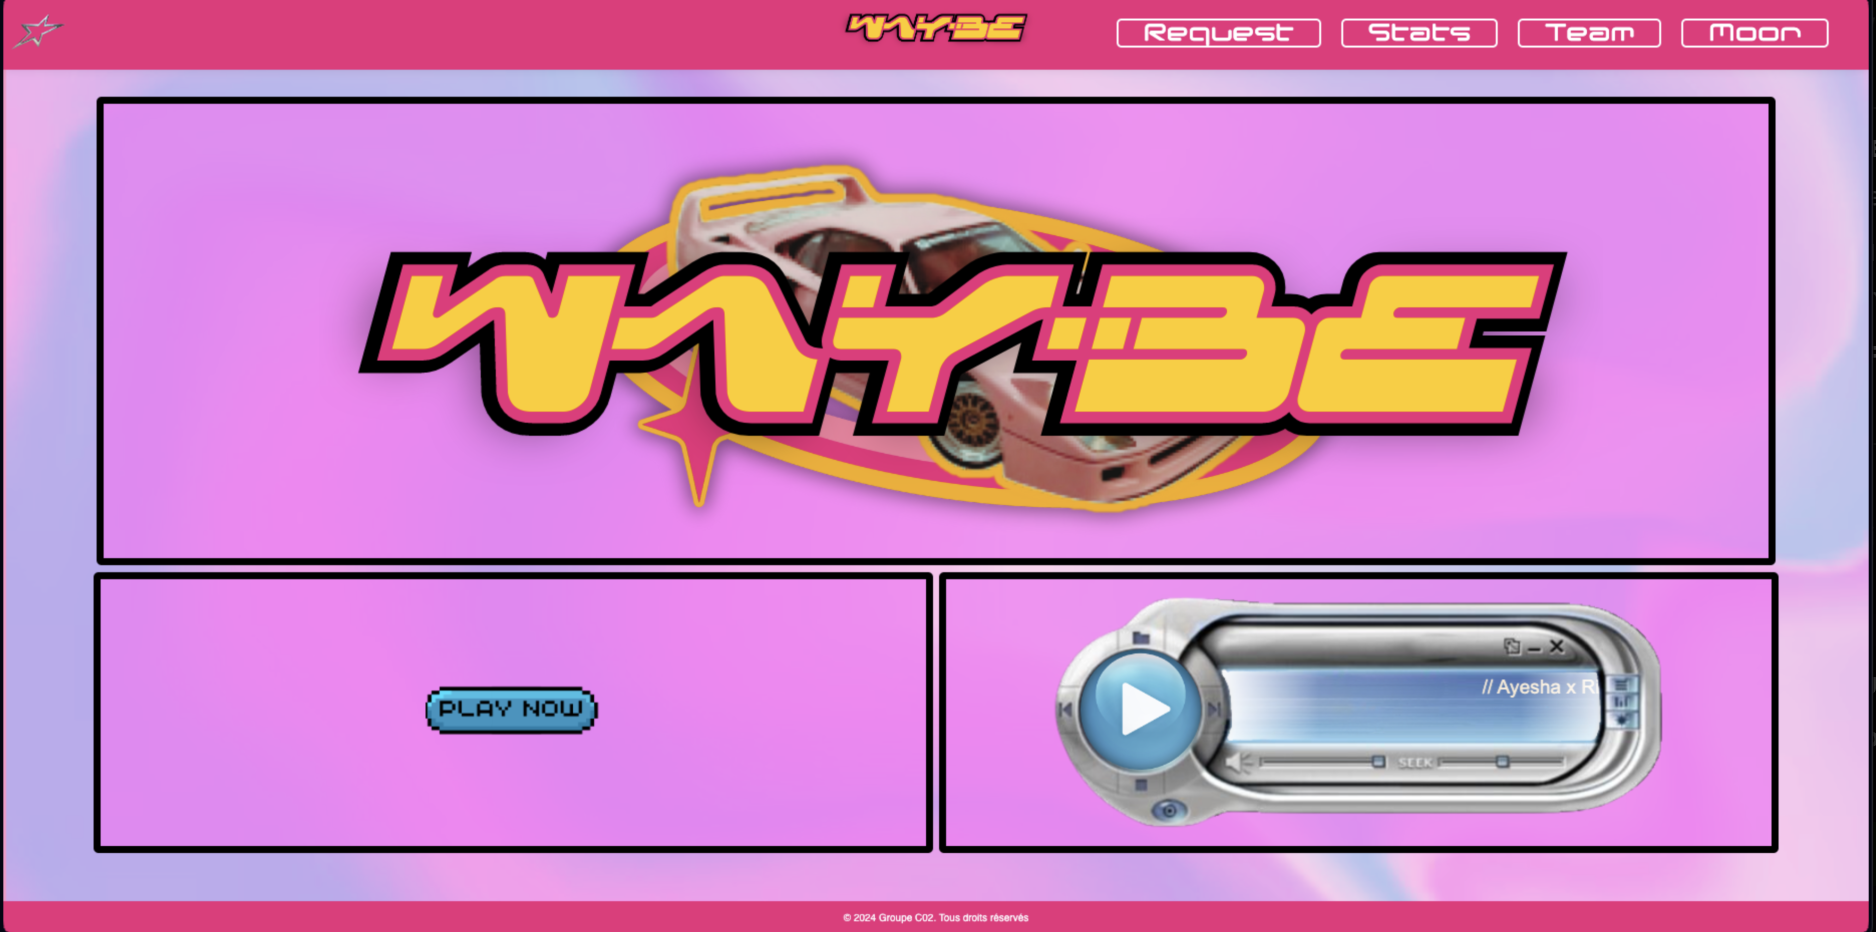
\includegraphics[scale=0.5]{logo/h.png}
\end{center}

Voici la page d'accueil de notre site, qui accueille nos utilisateurs. Elle comporte notre logo en gros, ainsi qu'une barre de navigation permettant de naviguer entre les différentes pages de WAY-BE. Chaque encadré blanc redirige vers une page en particulier que nous allons vous présenter dans un instant. Ensuite, dans l'encadré en bas à droite, nous avons implémenté un lecteur MP3 pour une référence aux années 2000. Il est totalement fonctionnel : vous pouvez appuyer sur play et écouter une musique libre de droit sur le thème des années 2000. Si cela vous ennuie, vous pouvez simplement mettre pause.
Rediregeons nous mtn vers la page Team pour une bref présentation de notre équipe . 

\section{Team page}
\begin{center}
    \includegraphics[scale=0.3]{logo/team.png}
\end{center}

Nous voici sur notre page Team. Nous avons opté pour une présentation inspirée des cartes Pokémon. Ces cartes peuvent être retournées, je vous invite à aller directement les tester sur notre site. Chaque écriture en mandarin représente le poste de chacun au sein de l'équipe. Maintenant, faisons un petit détour vers la lune avec la page Moon.


\section{Moon page}
\begin{center}
    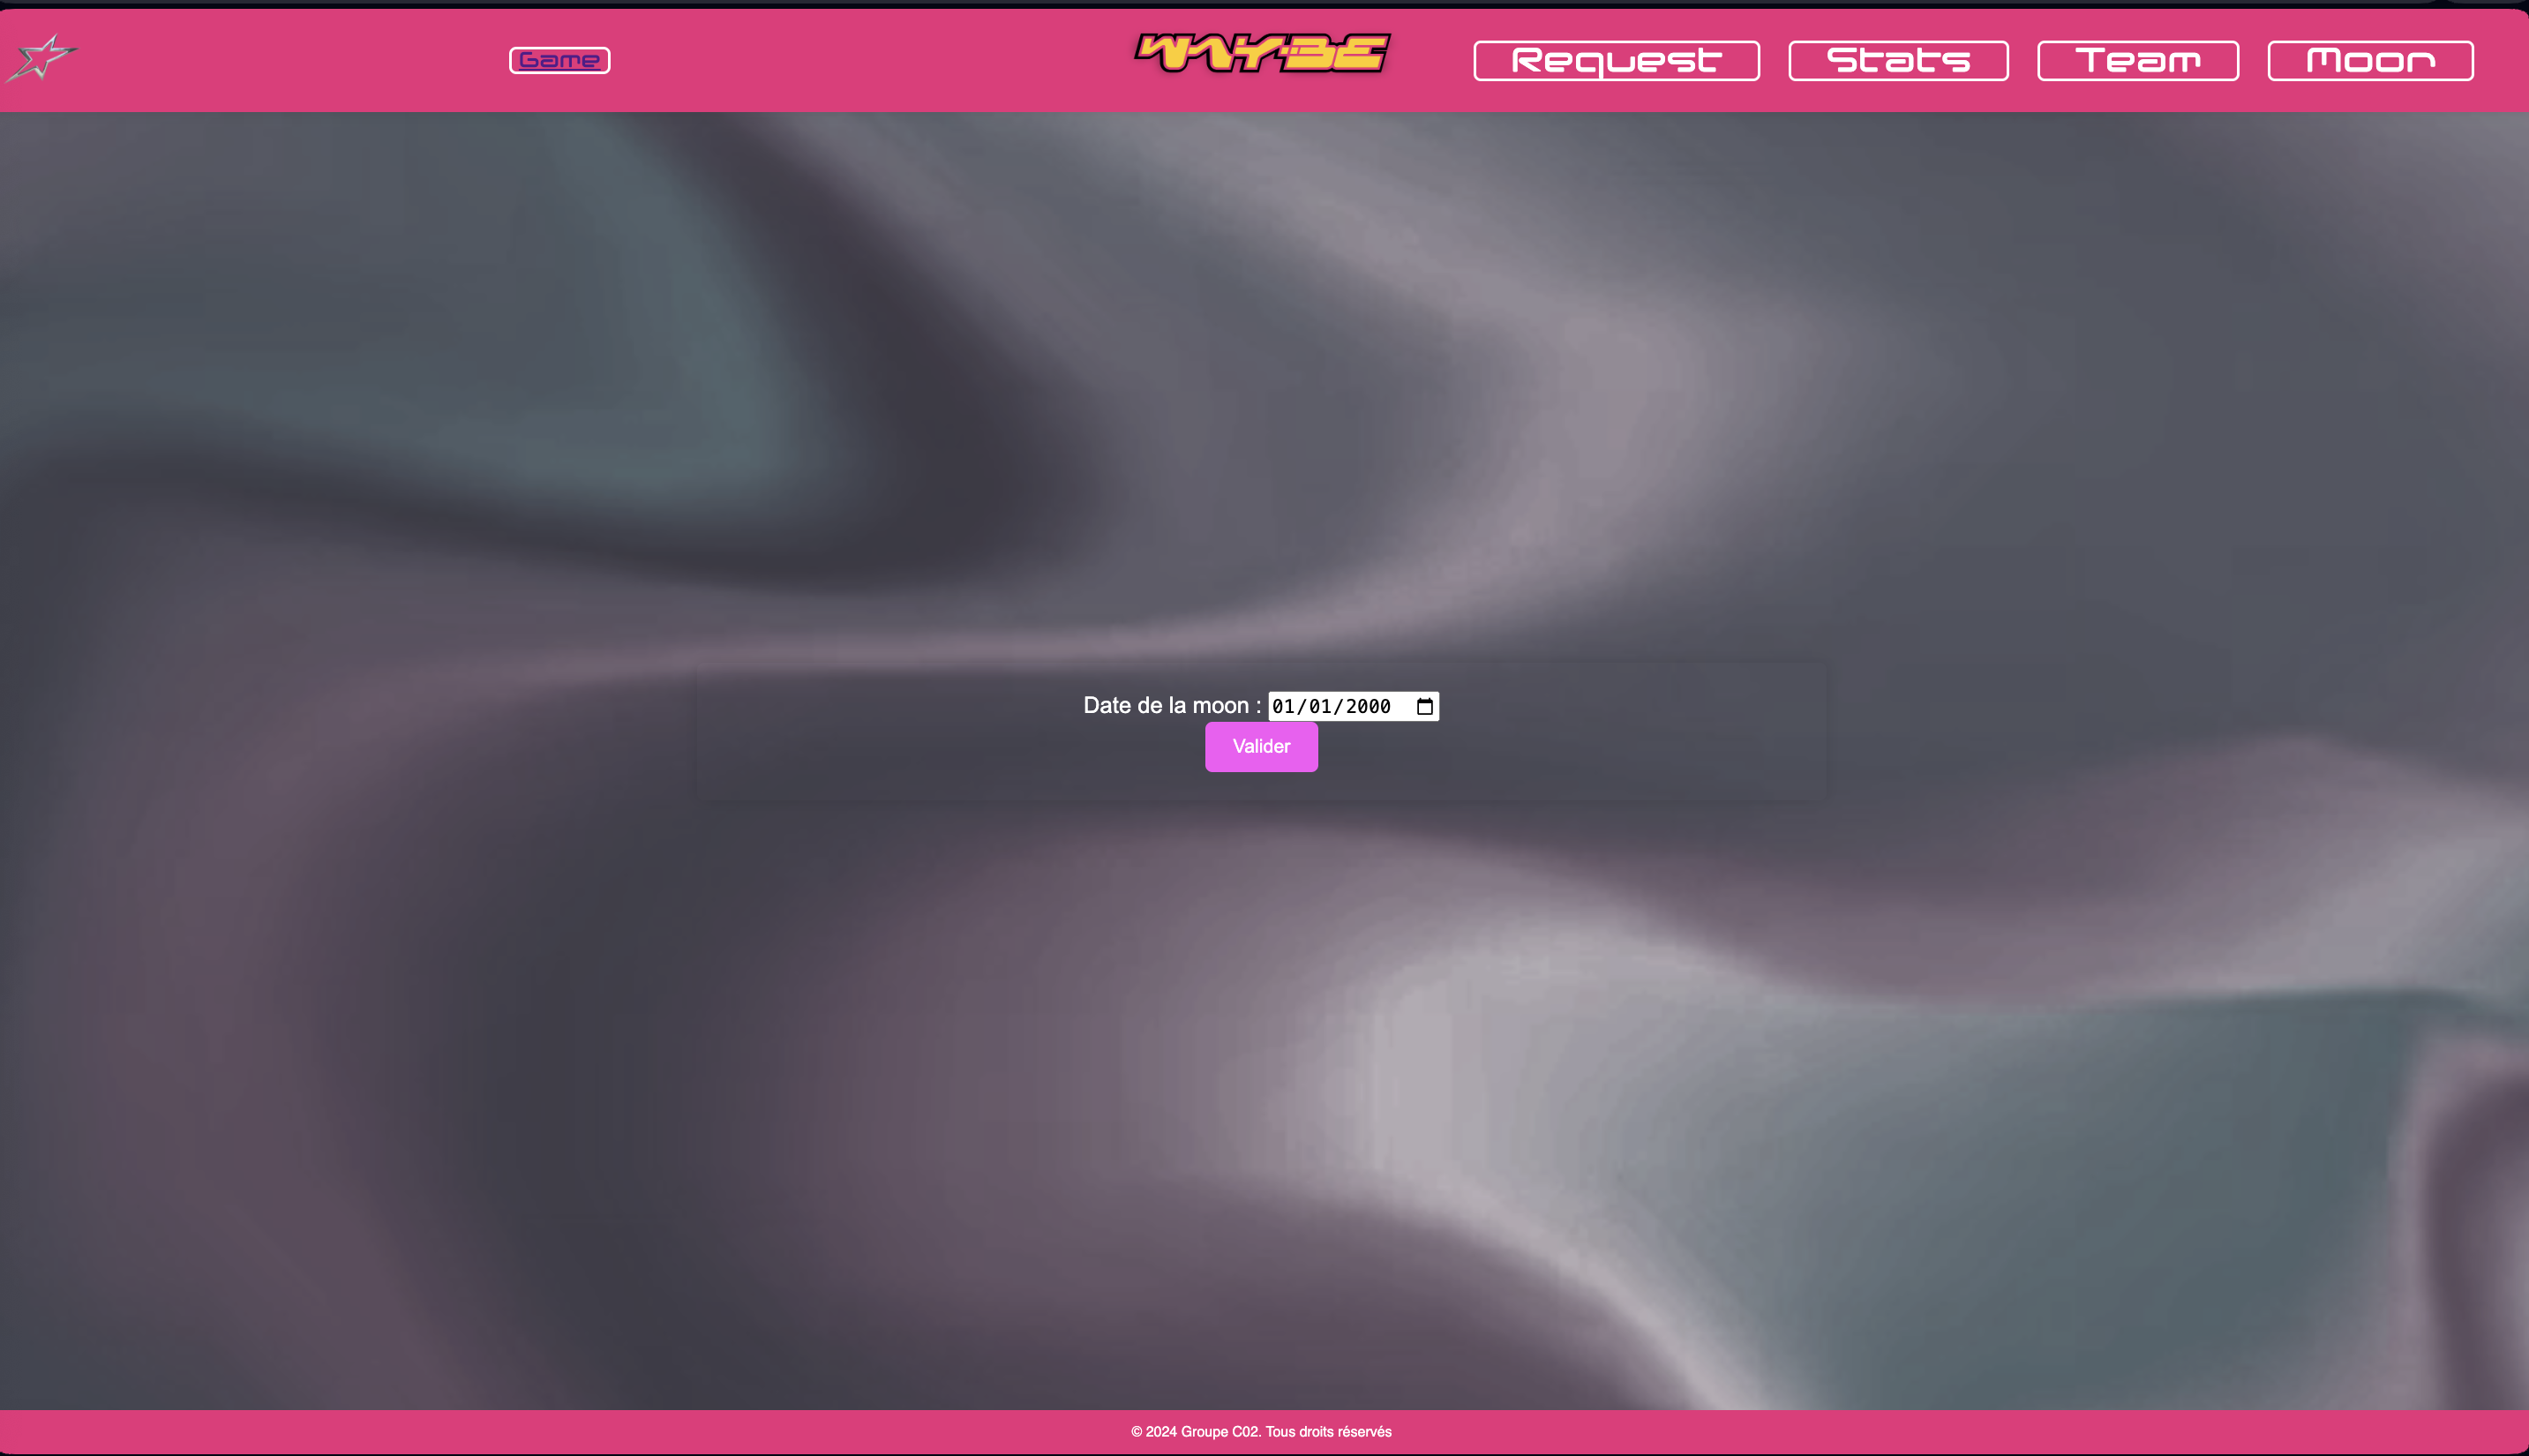
\includegraphics[scale=0.3]{logo/MOON1.png}
\end{center}

Nous voici sur la Lune, enfin presque. Il faut d'abord spécifier la date à laquelle nous voulons connaître la phase de la lune. Ici, nous avons choisi le 01/01/2000.

\begin{center}
    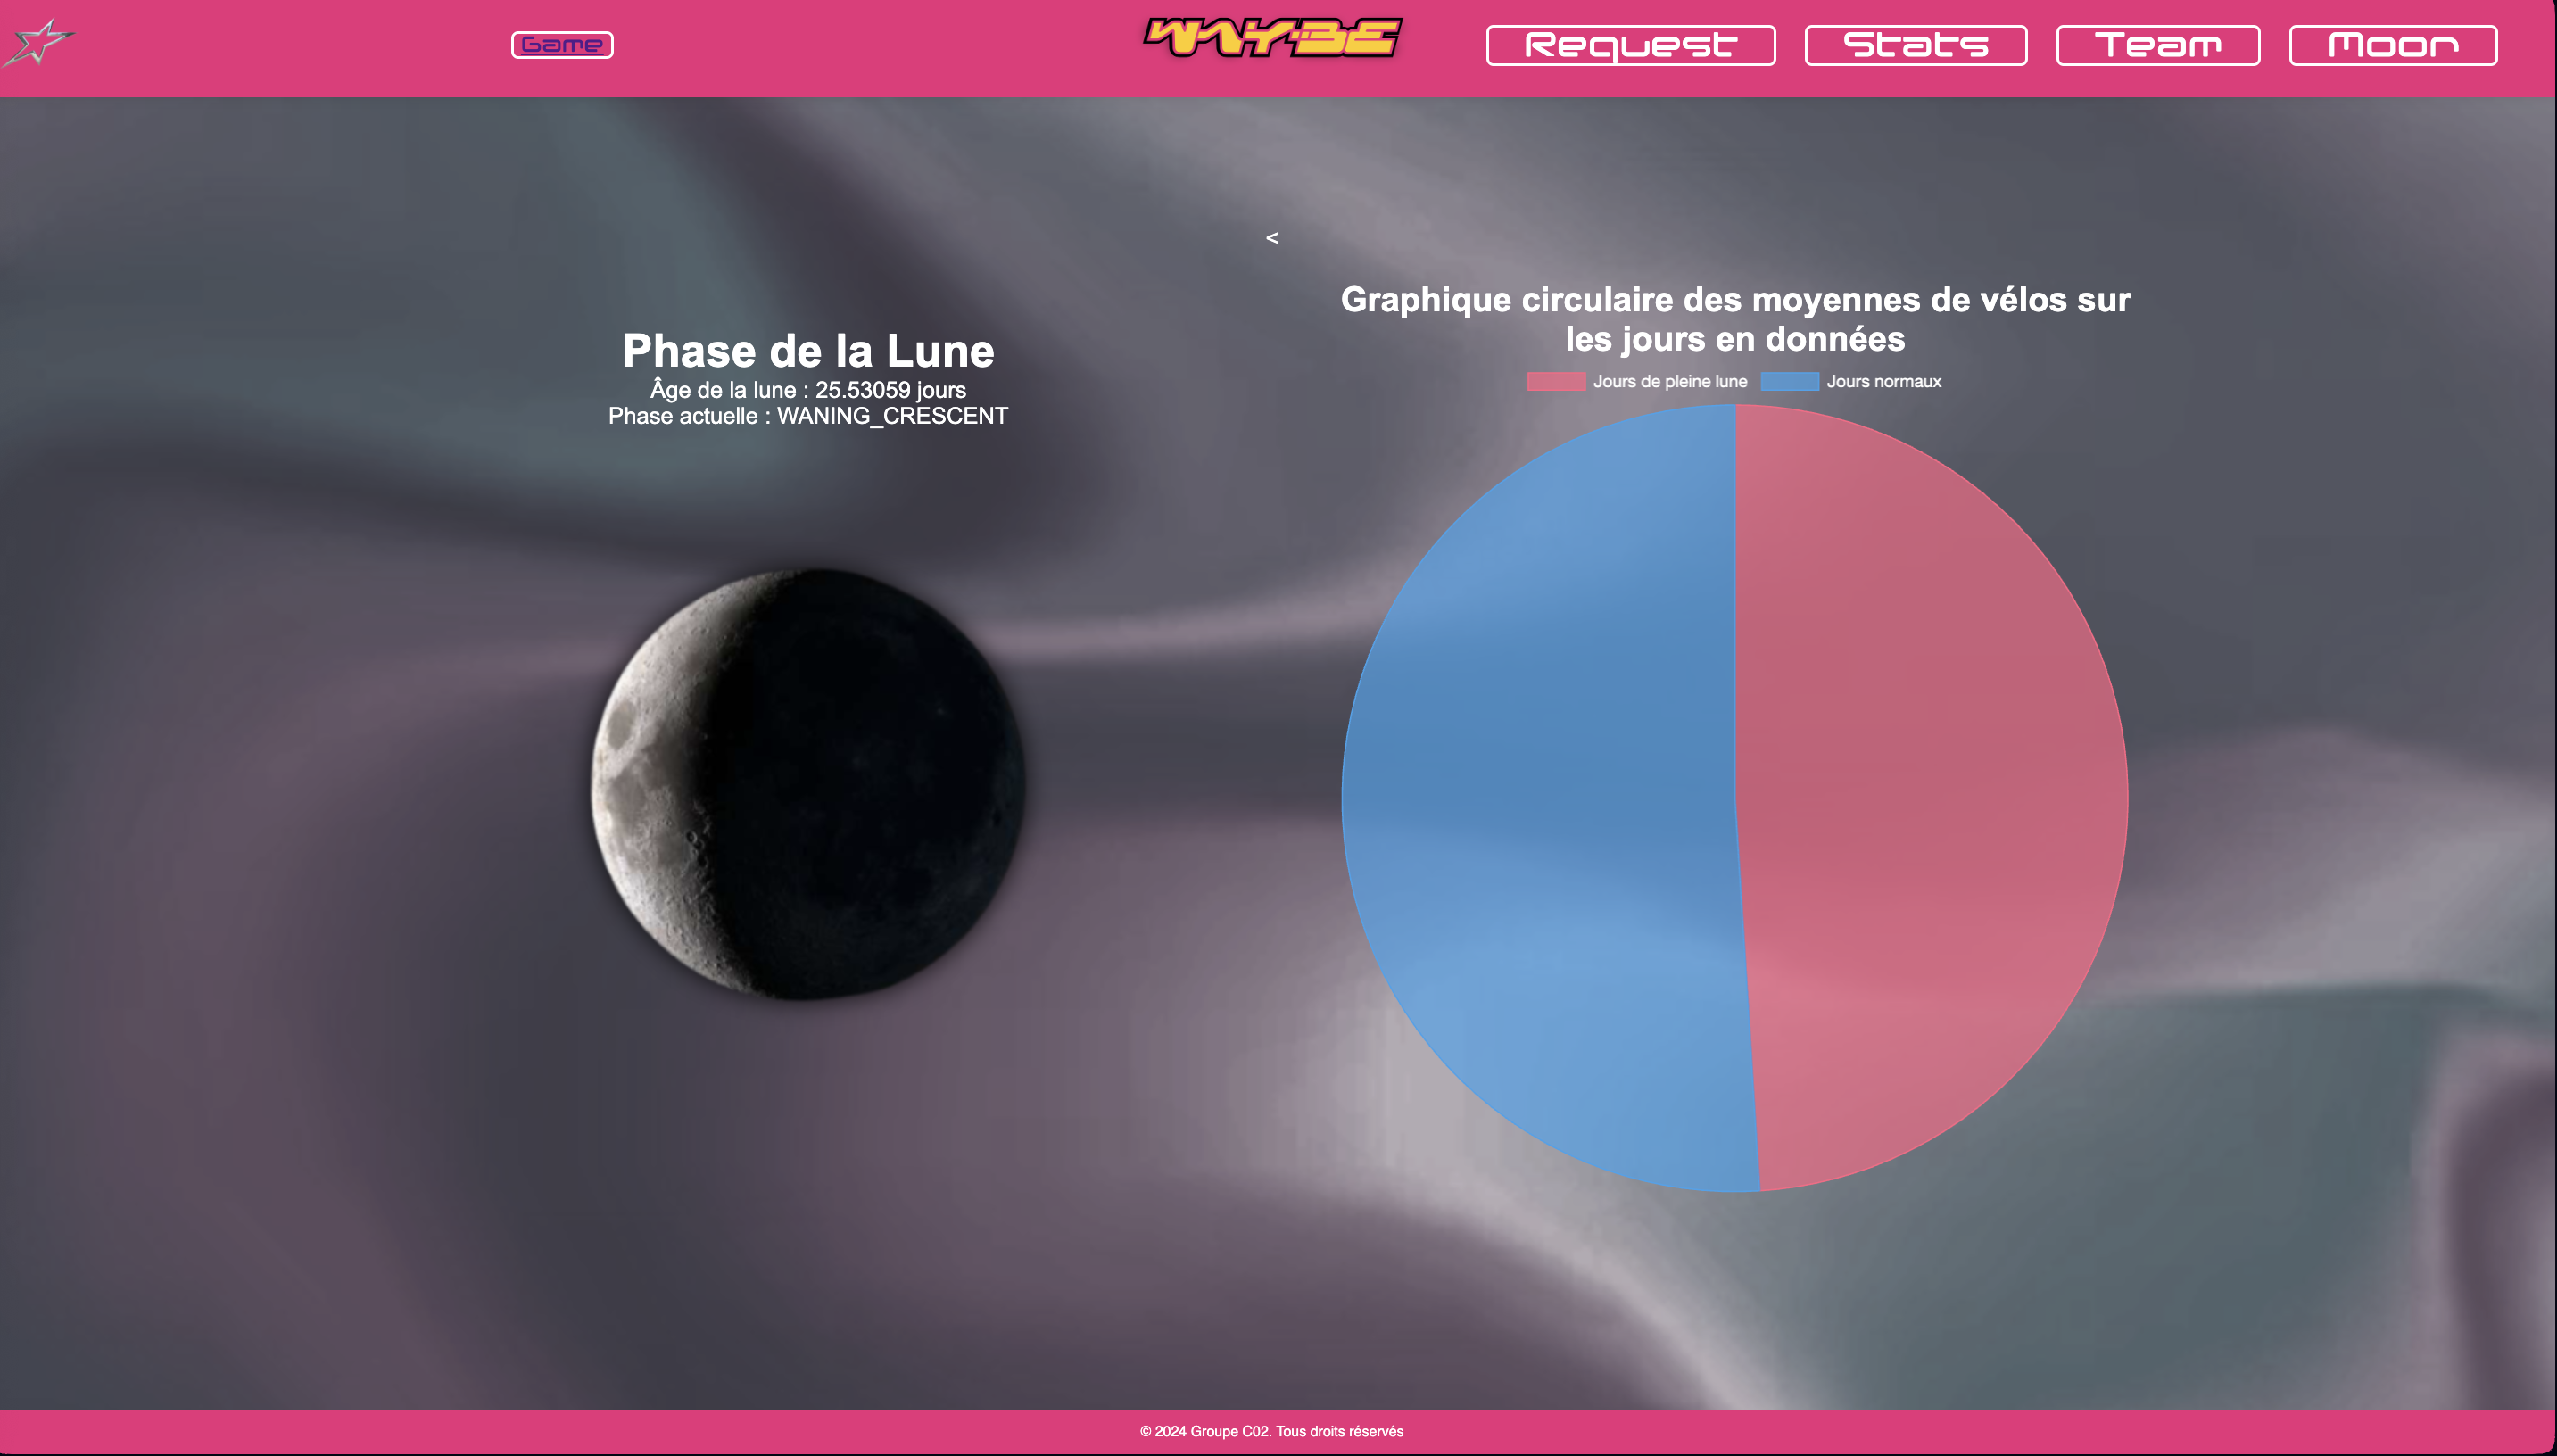
\includegraphics[scale=0.3]{logo/MOON2.png}
\end{center}

Nous voilà enfin sur la lune. Ici, nous pouvons voir la phase de la lune à la date demandée, ainsi qu'un graphique circulaire sur les moyennes des vélos sur les jours de données (en jours de pleine lune ou non). Nous avons choisi le graphique circulaire pour rester dans le thème de l'espace et aussi parce qu'il est plus facile de voir que c'est presque équivalent.
\subsection{Tests de Moon}
    Comment avons-nous testé notre fonction pour calculer les phases de lune, que ce soit du début de notre ère à sa fin, toujours pas programmé

\begin{itemize}
    \item En premier lieu, nous avons testé la fonction qui calcule la moyenne de vélos les jours de pleine lune ou pas en effectuant des tests unitaires basiques. Cela consistait à injecter différentes données pour lesquelles nous connaissions déjà la réponse, afin de vérifier si la fonction nous renvoyait les résultats attendus. \\

     \item Pour les phases de lune, nous avons récupéré des données d'un site spécialisé dans les phases de lune et les avons comparées avec les résultats de notre fonction. Nous avons effectué plus de 15 tests différents pour vérifier la précision de notre fonction. Et tous les tests ont conclut que nos tests passaient à 96\%.\\
\end{itemize}

Maintenant, que diriez-vous d'aller faire des recherches plus spécifiques dans notre page request ?

\section{Request page}

\begin{center}
    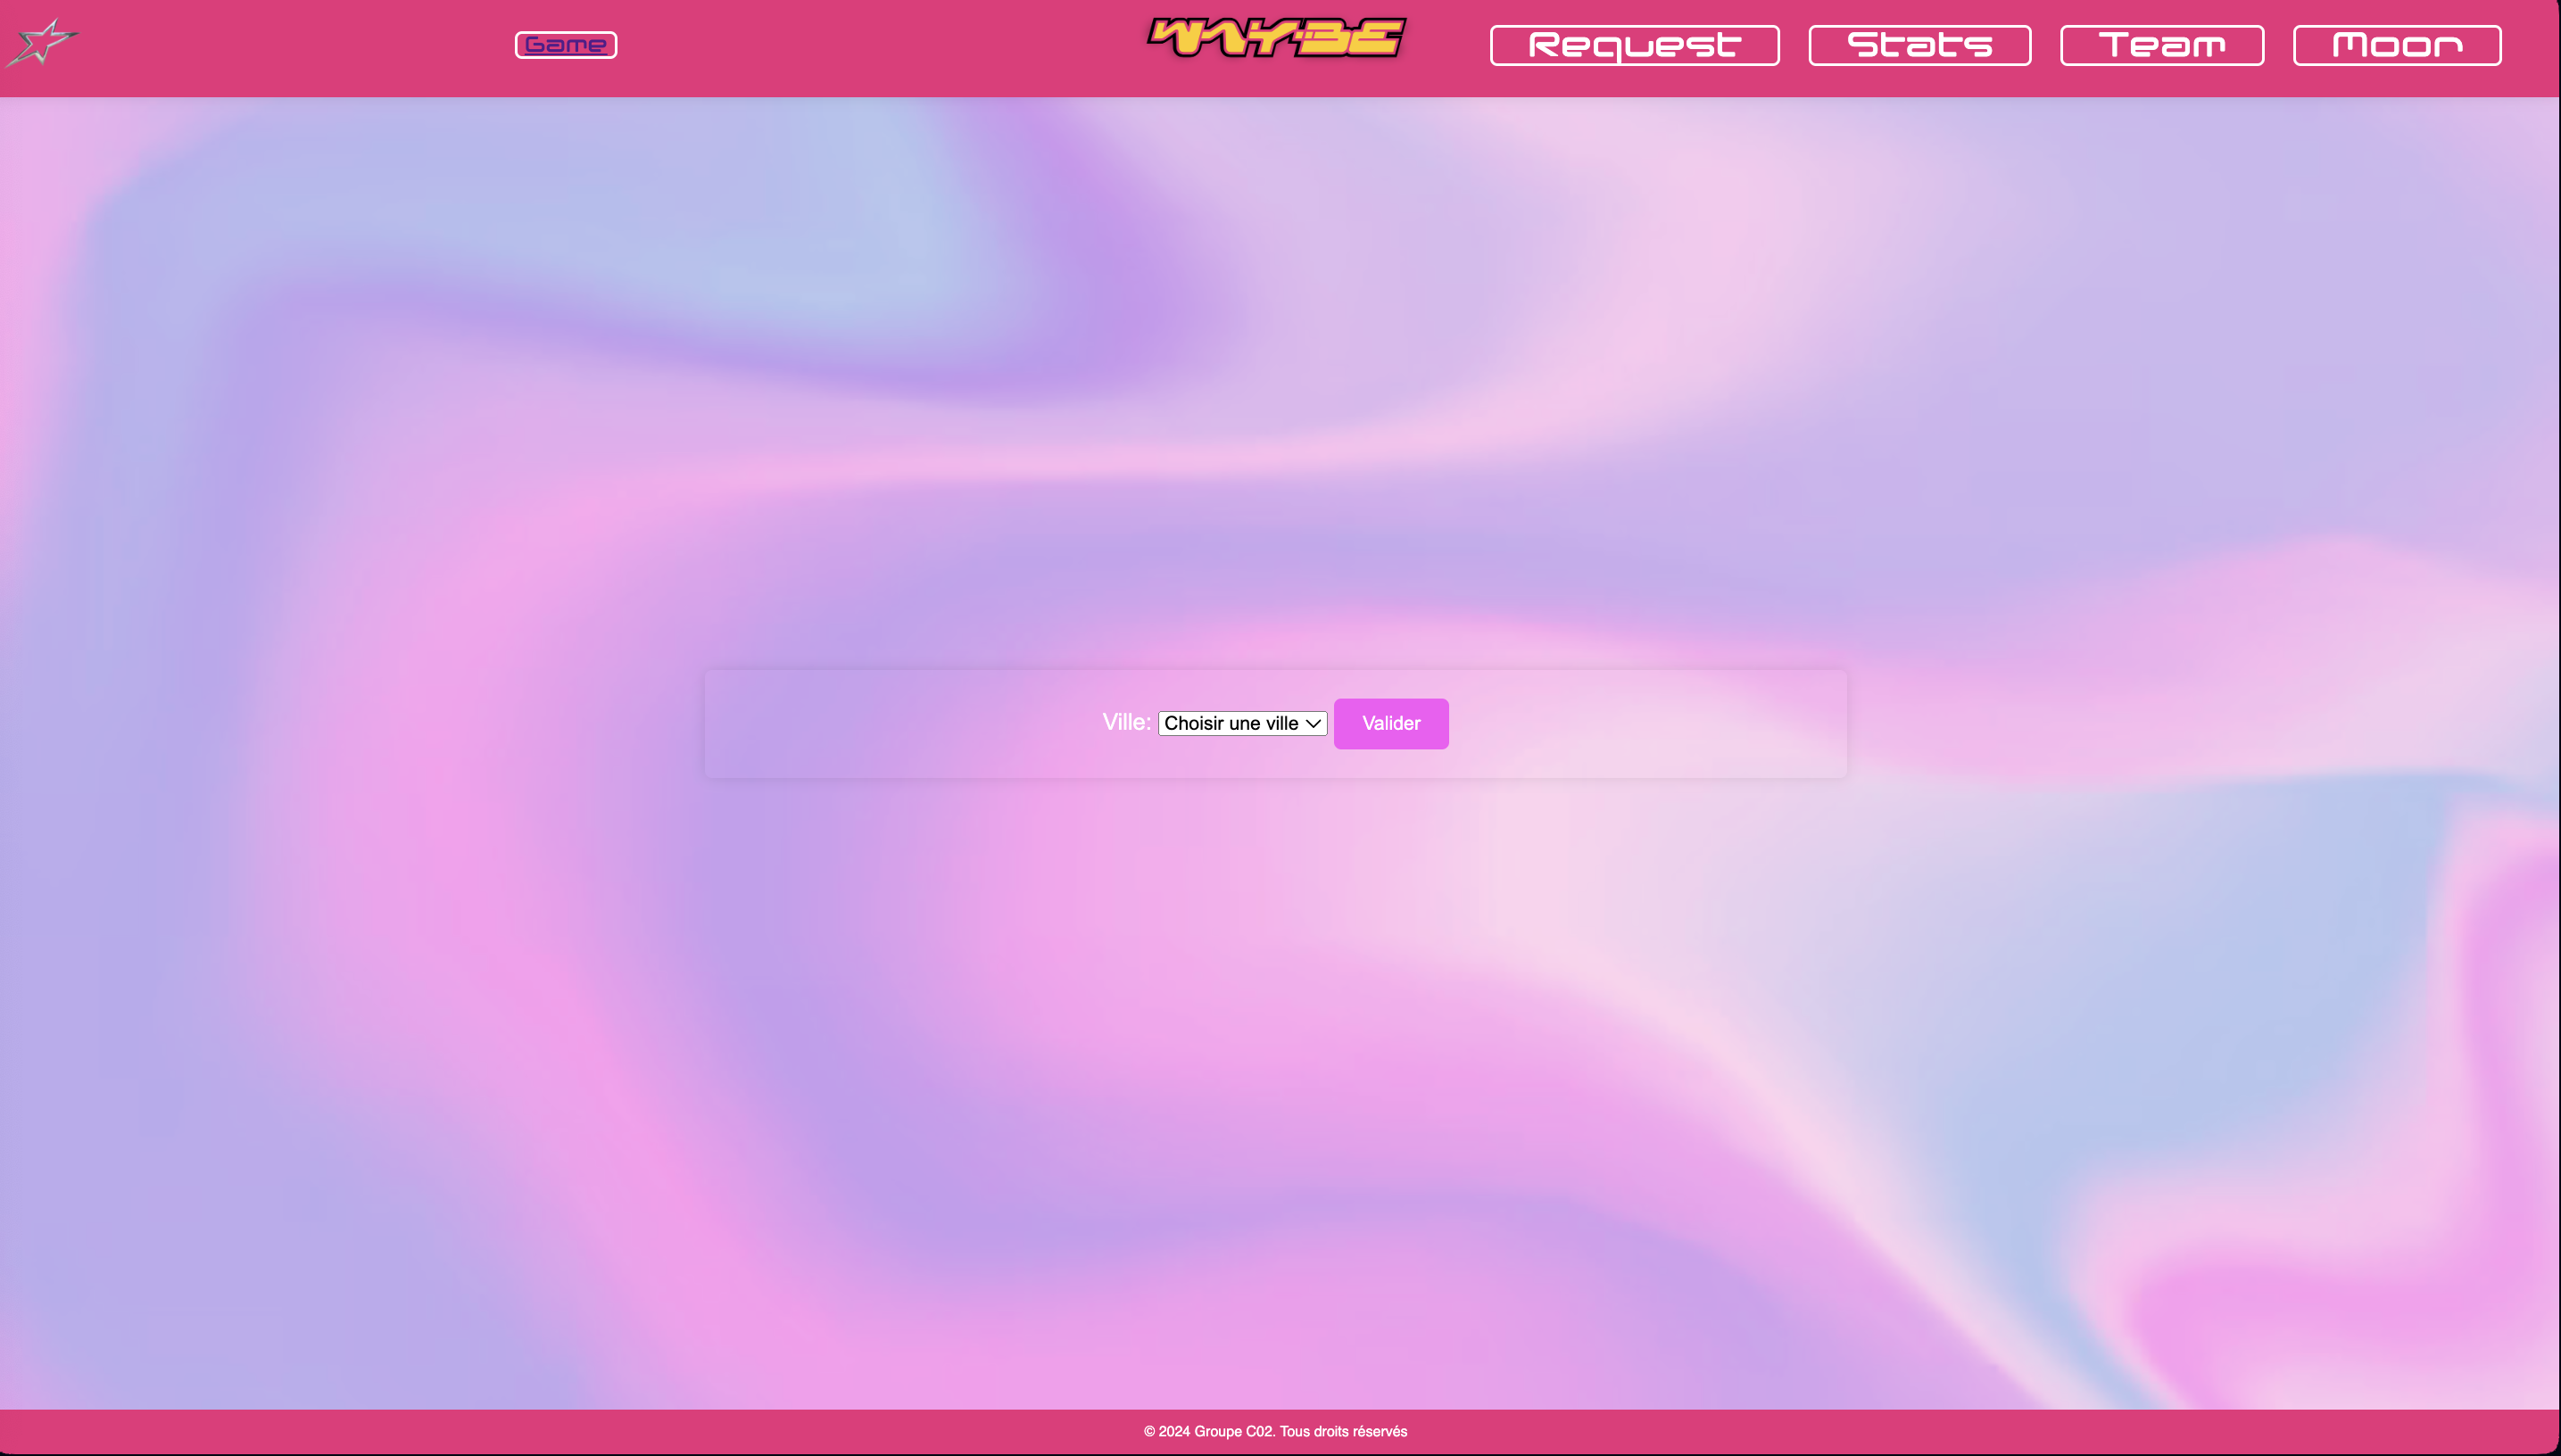
\includegraphics[scale=0.3]{logo/request.png}
\end{center}

En tout premier lieu, choisissons une ville.
prenons Charleroi

\begin{center}
    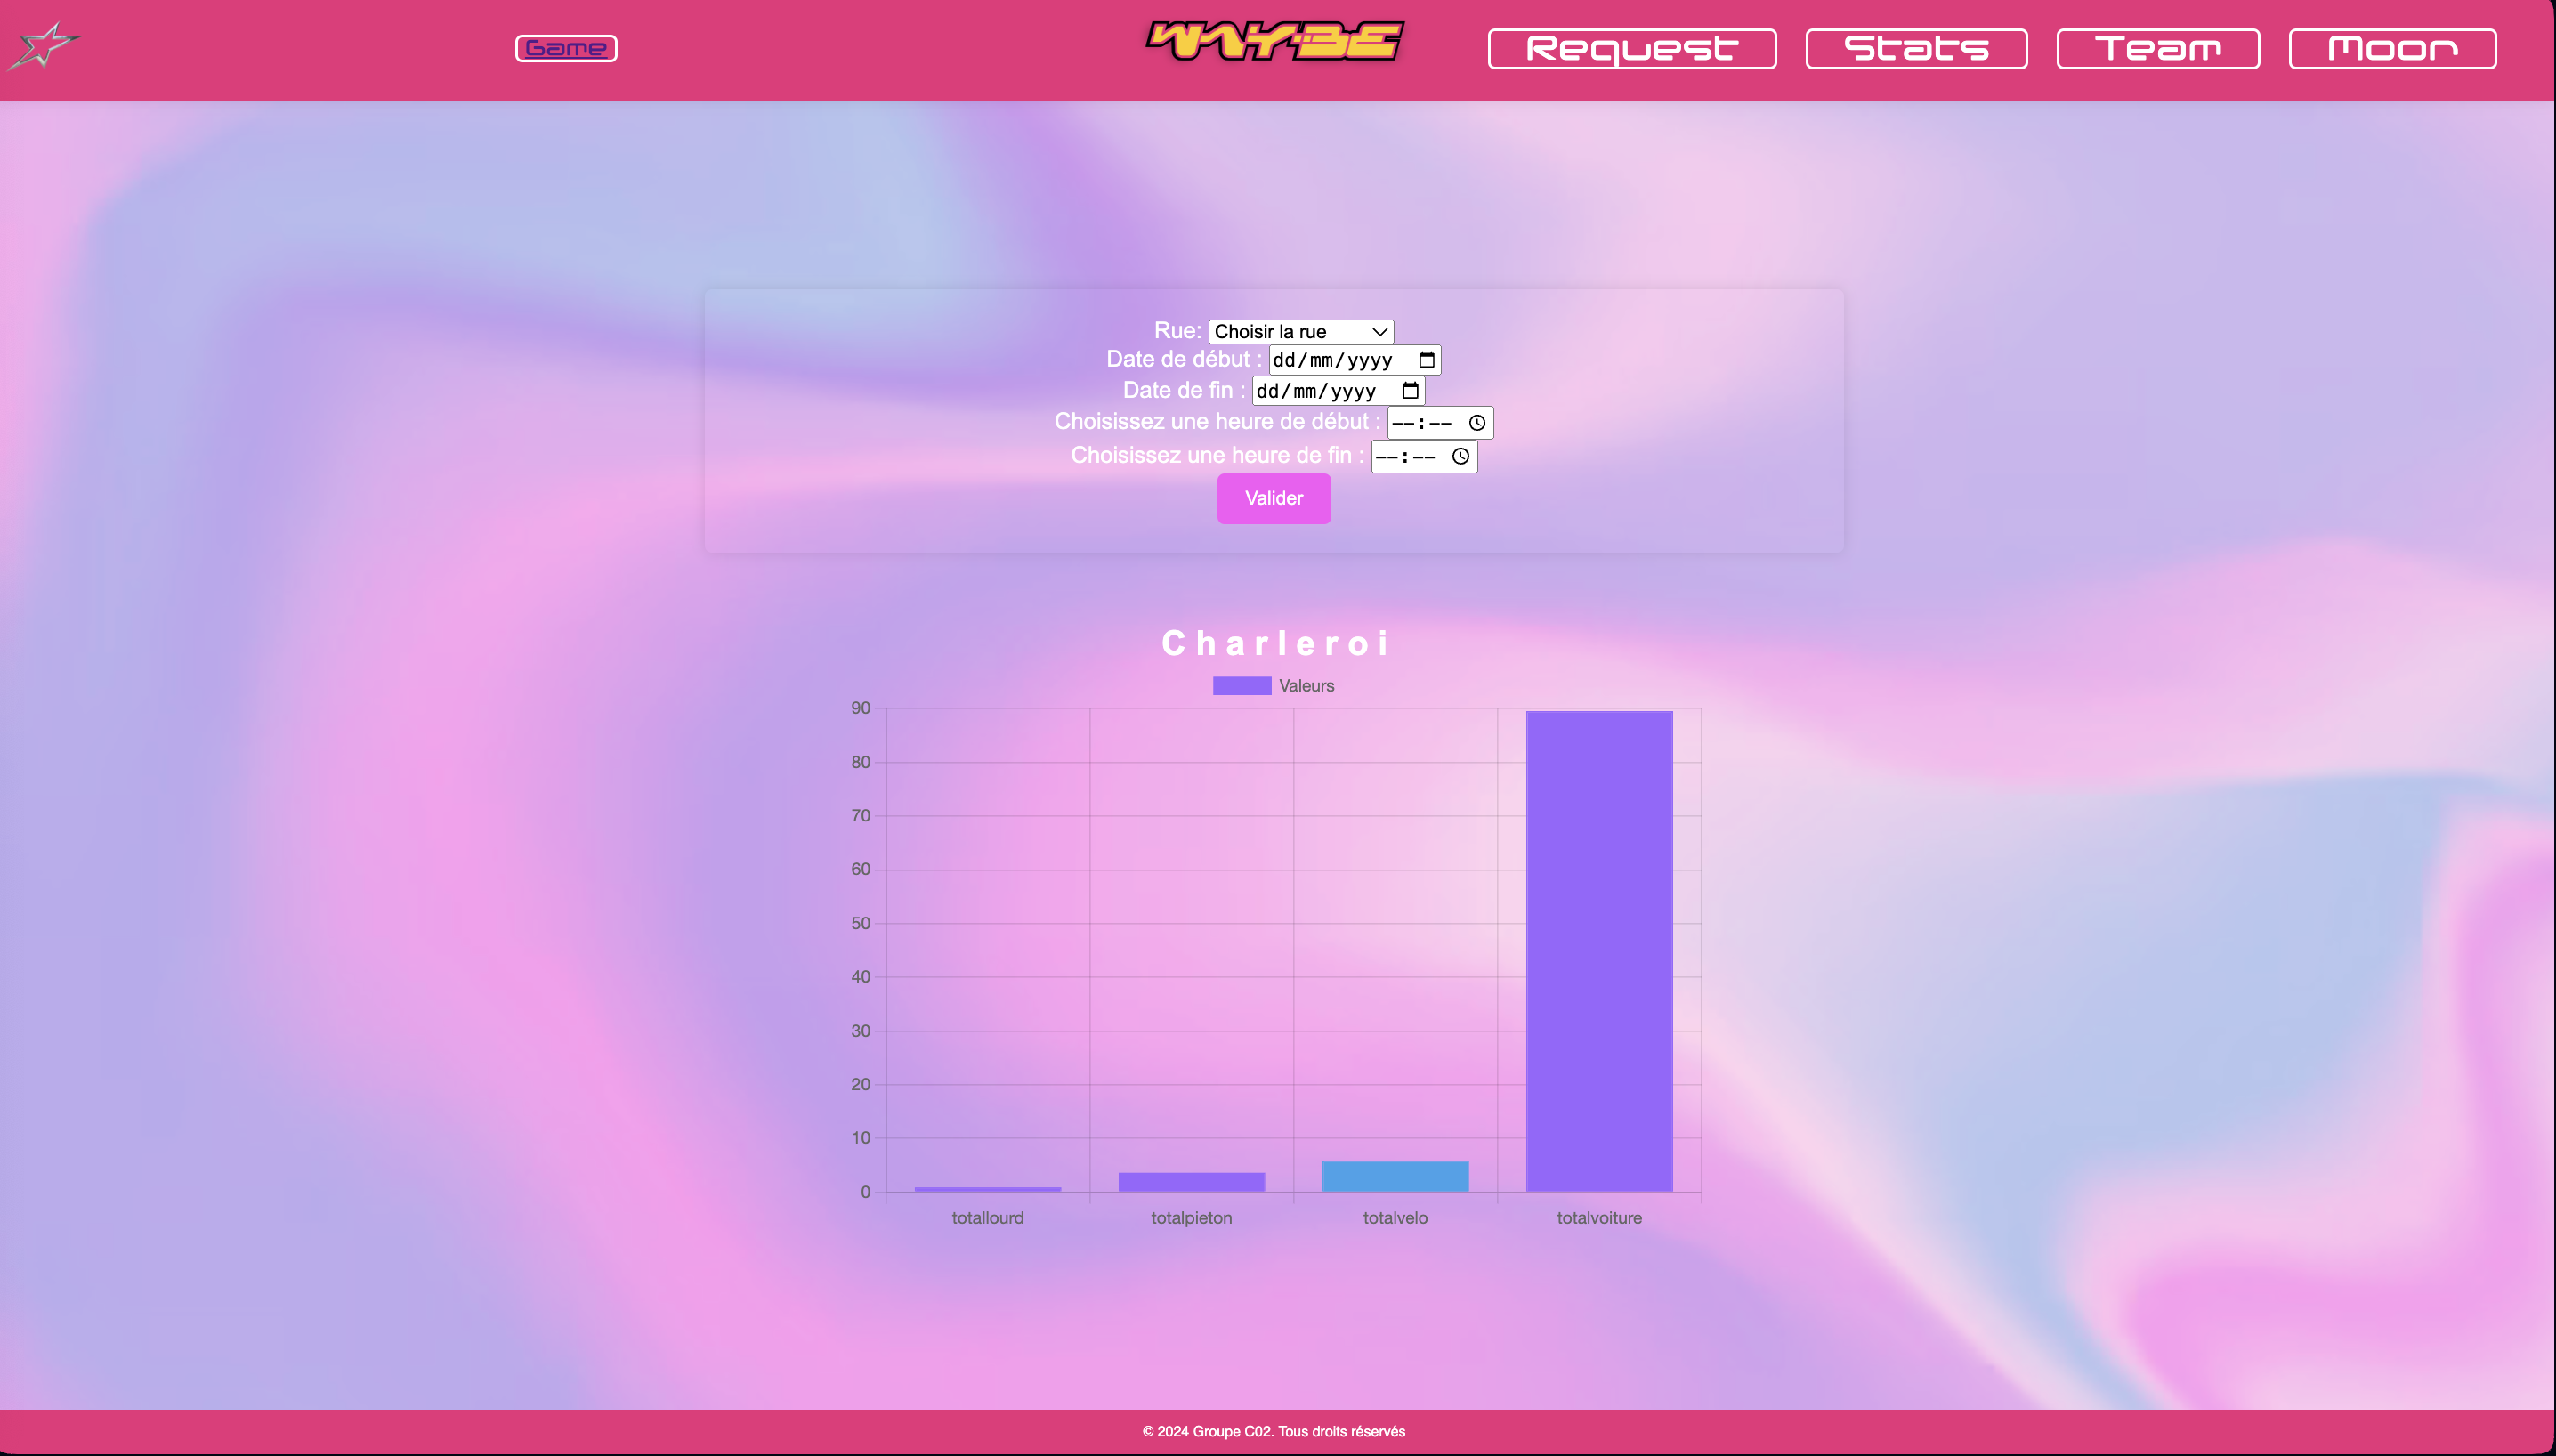
\includegraphics[scale=0.3]{logo/Request_c.png}
\end{center}

Nous pouvons voir un graphique en bâtons qui nous donne des informations sur la ville de Charleroi, telles que le nombre de poids lourds, de voitures, de vélos et de piétons dans la ville. Le choix d'un graphique en bâtons a été fait pour faciliter la visualisation des grandes différences de véhicules présents dans la ville.\\

Nous pouvons être plus spécifiques en choisissant la rue maintenant. Prenons le Boulevard Audent. avec une date entre le 31 décembre 2023 10H00 er le 1 janvier 2024 20h00 pour voir ce qu' il s'est passé pendant le nouvel an 

\begin{center}
    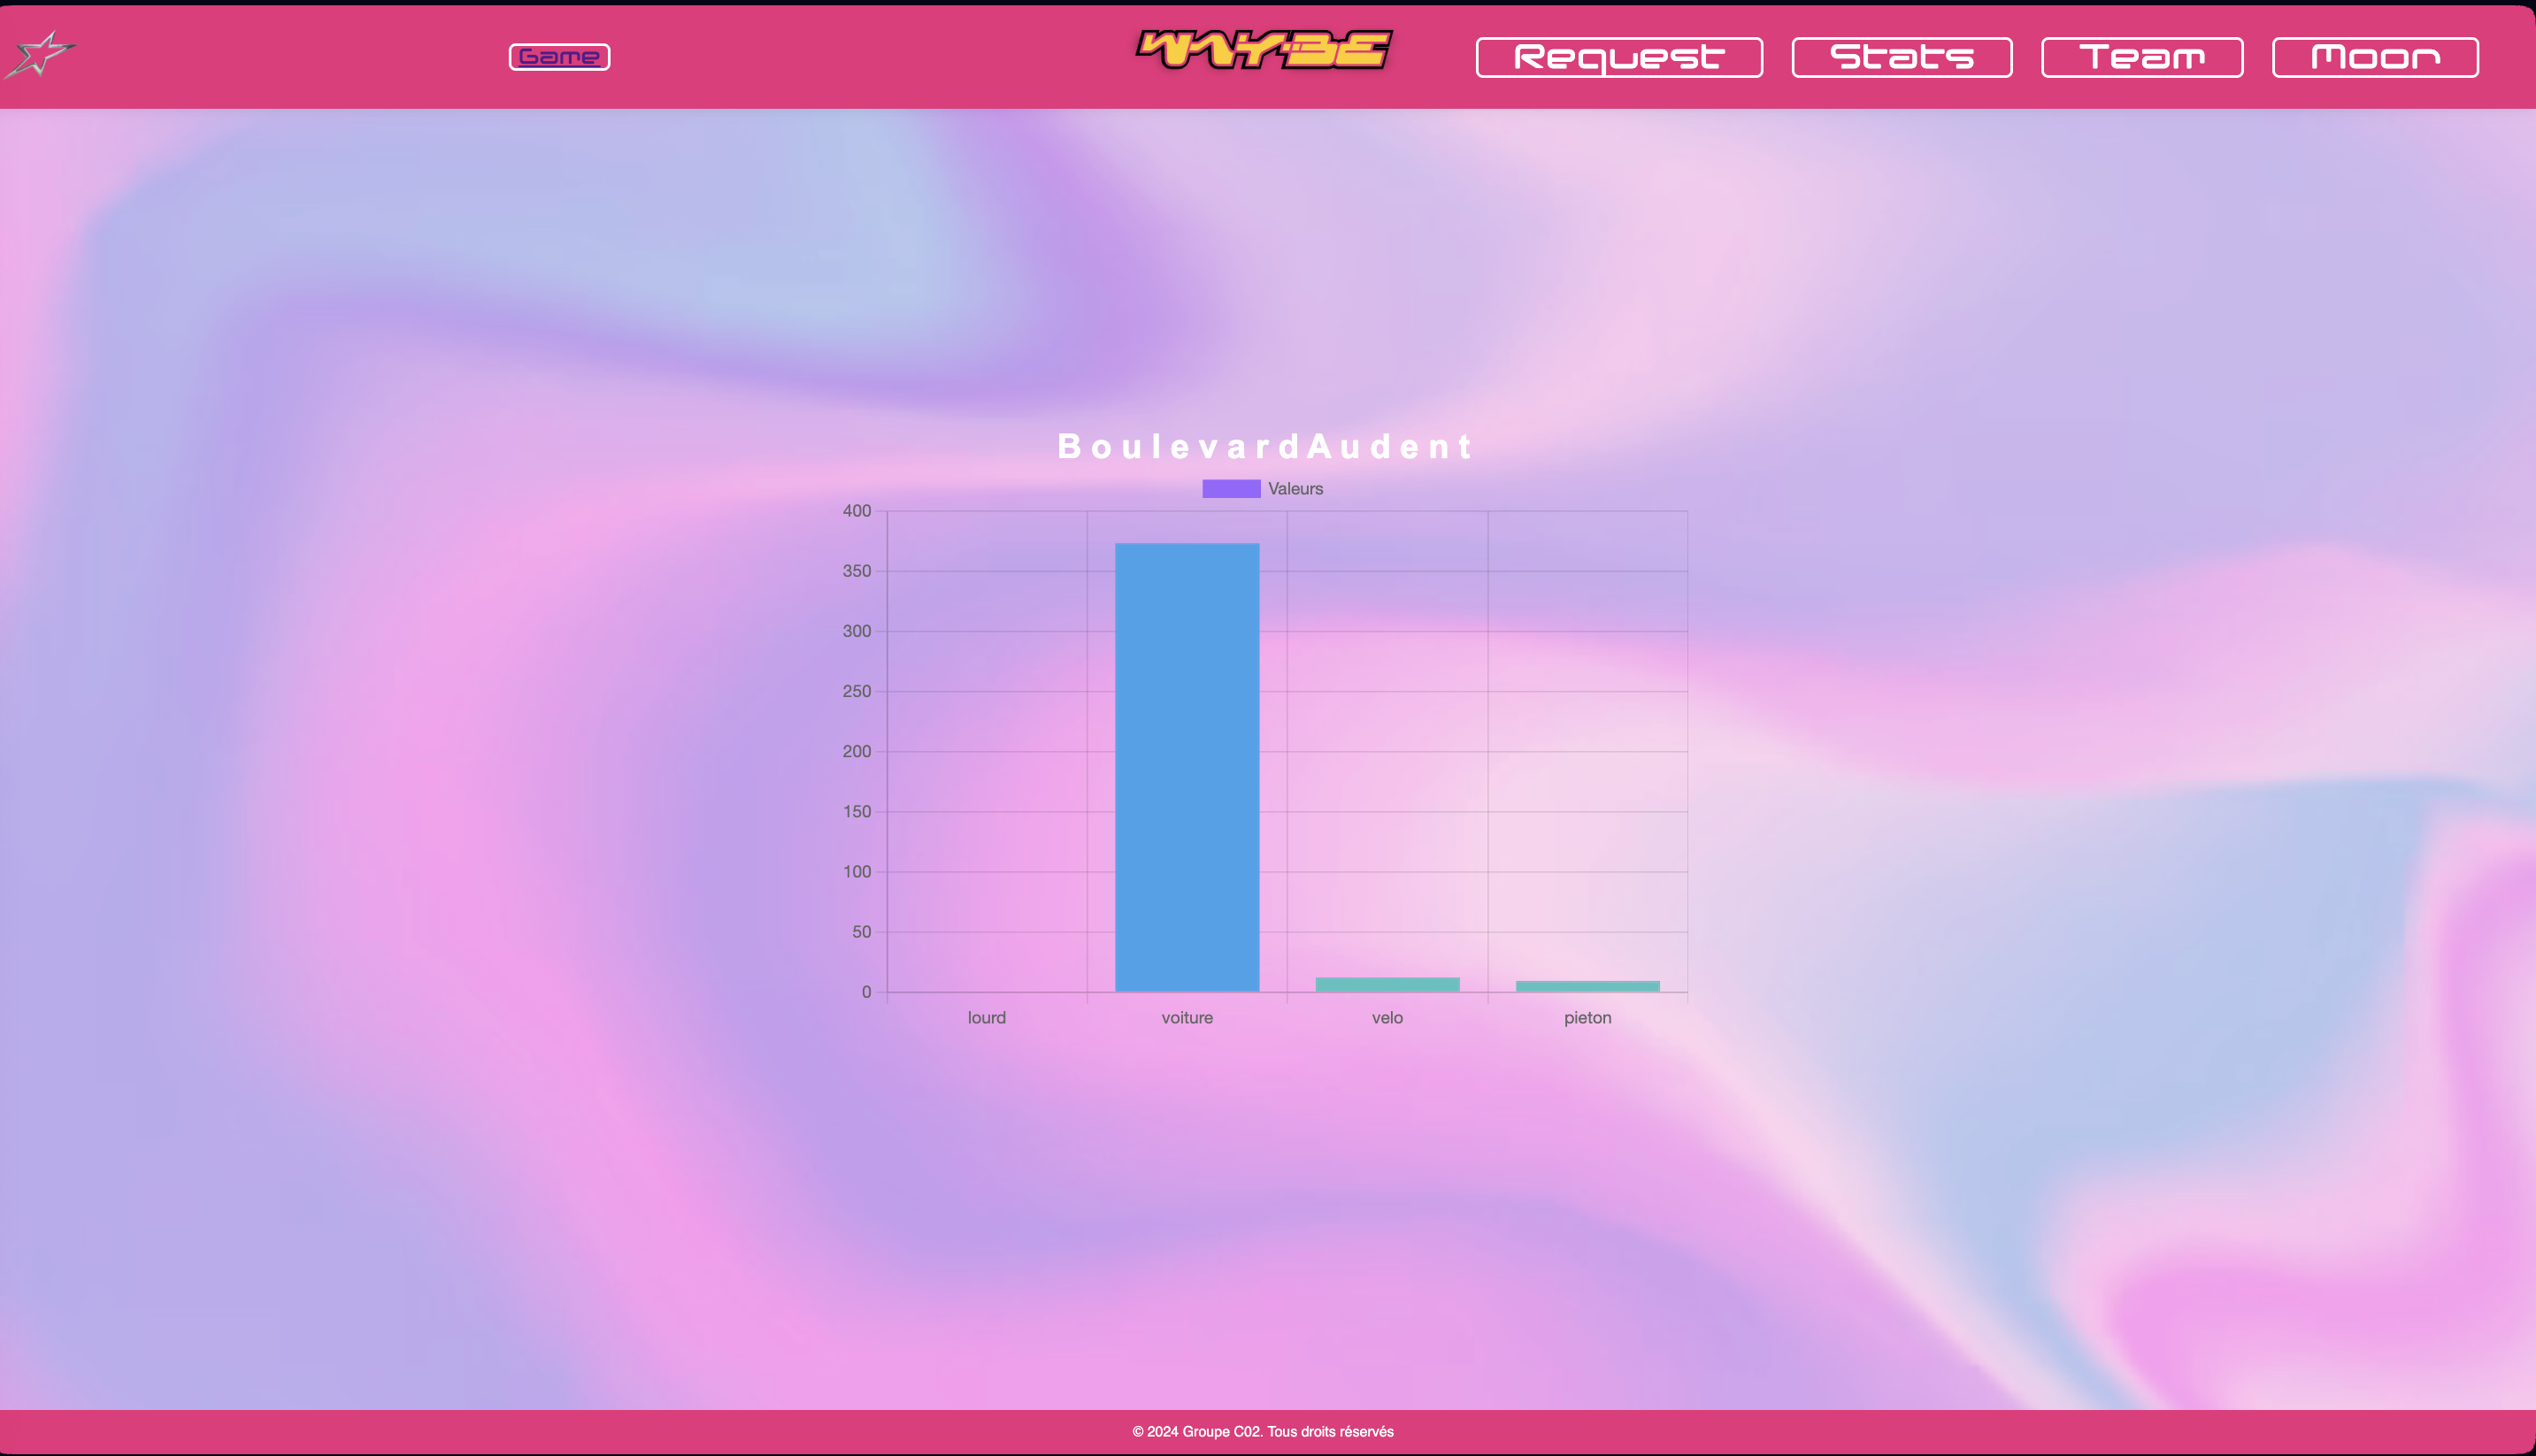
\includegraphics[scale=0.3]{logo/boulevard.png}
\end{center}

Et voilà les données des véhicules circulant durant le Nouvel An à Charleroi sur le Boulevard Audent. Nous avons choisi un graphe à bâtonnets pour la même raison que le précédent, et comme on peut le voir ici, les voitures ont beaucoup circulé ce jour-là. Passons maintenant au jeux notre fonction en plus . 


\section{Game page}
\begin{center}
    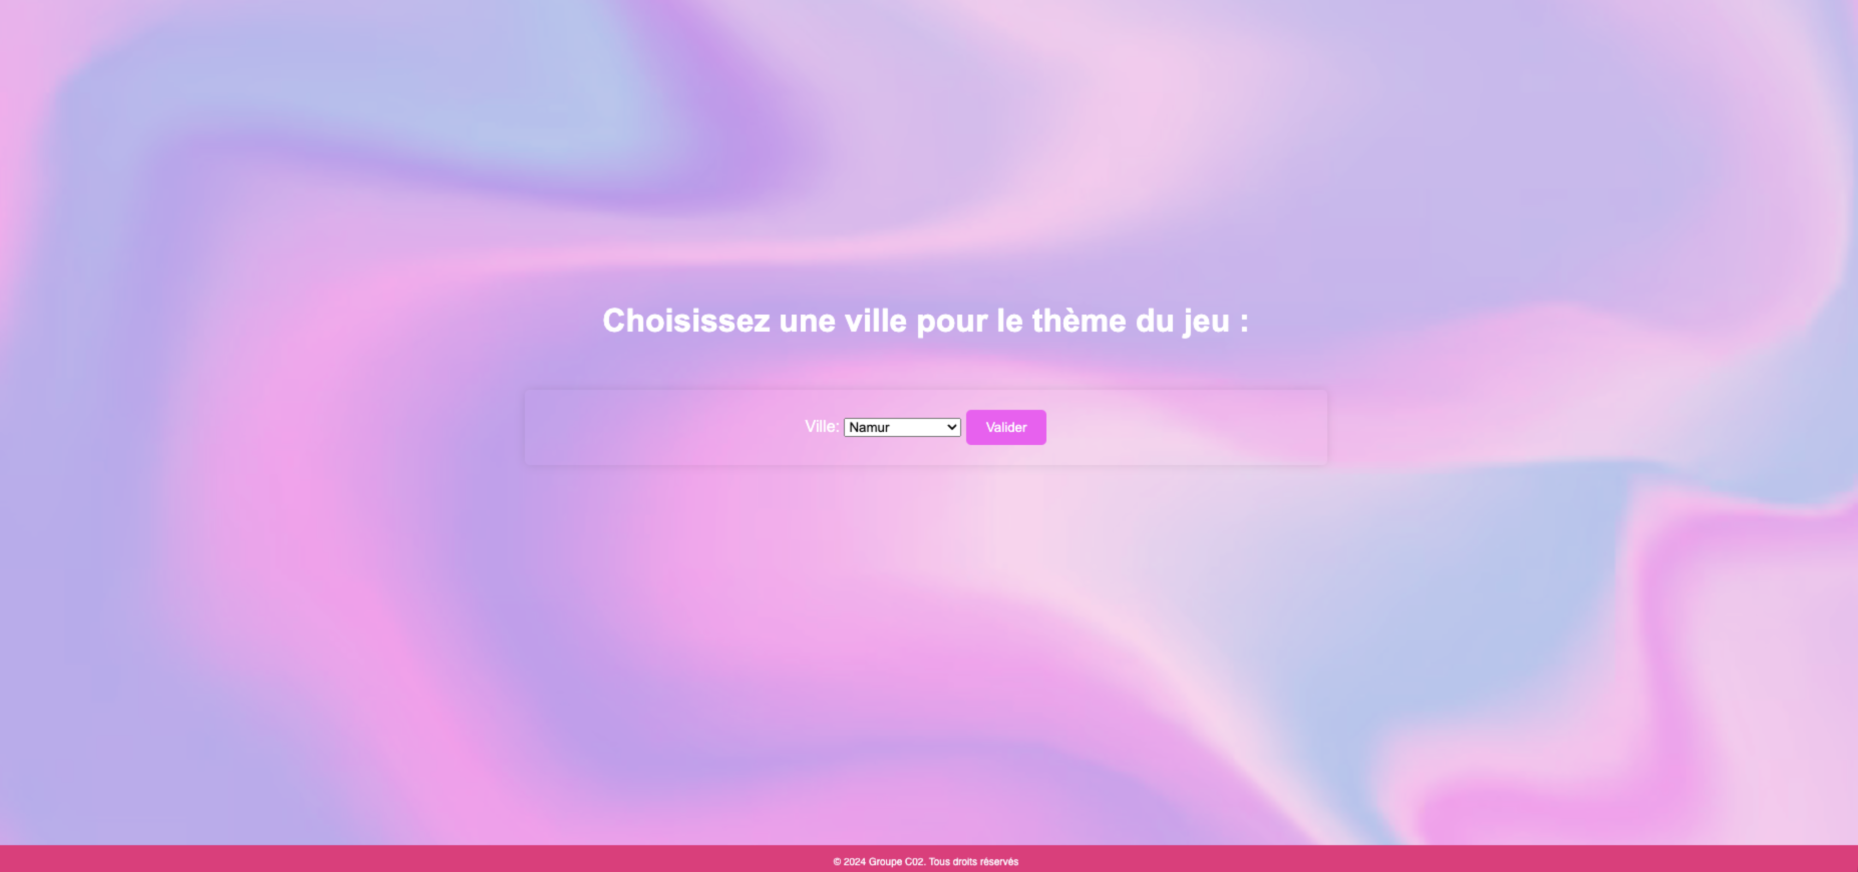
\includegraphics[scale=0.4]{logo/cho.png}
\end{center}

Ici, nous pouvons choisir la ville et le thème du jeu changera. Choisissons Namur.

\begin{center}
    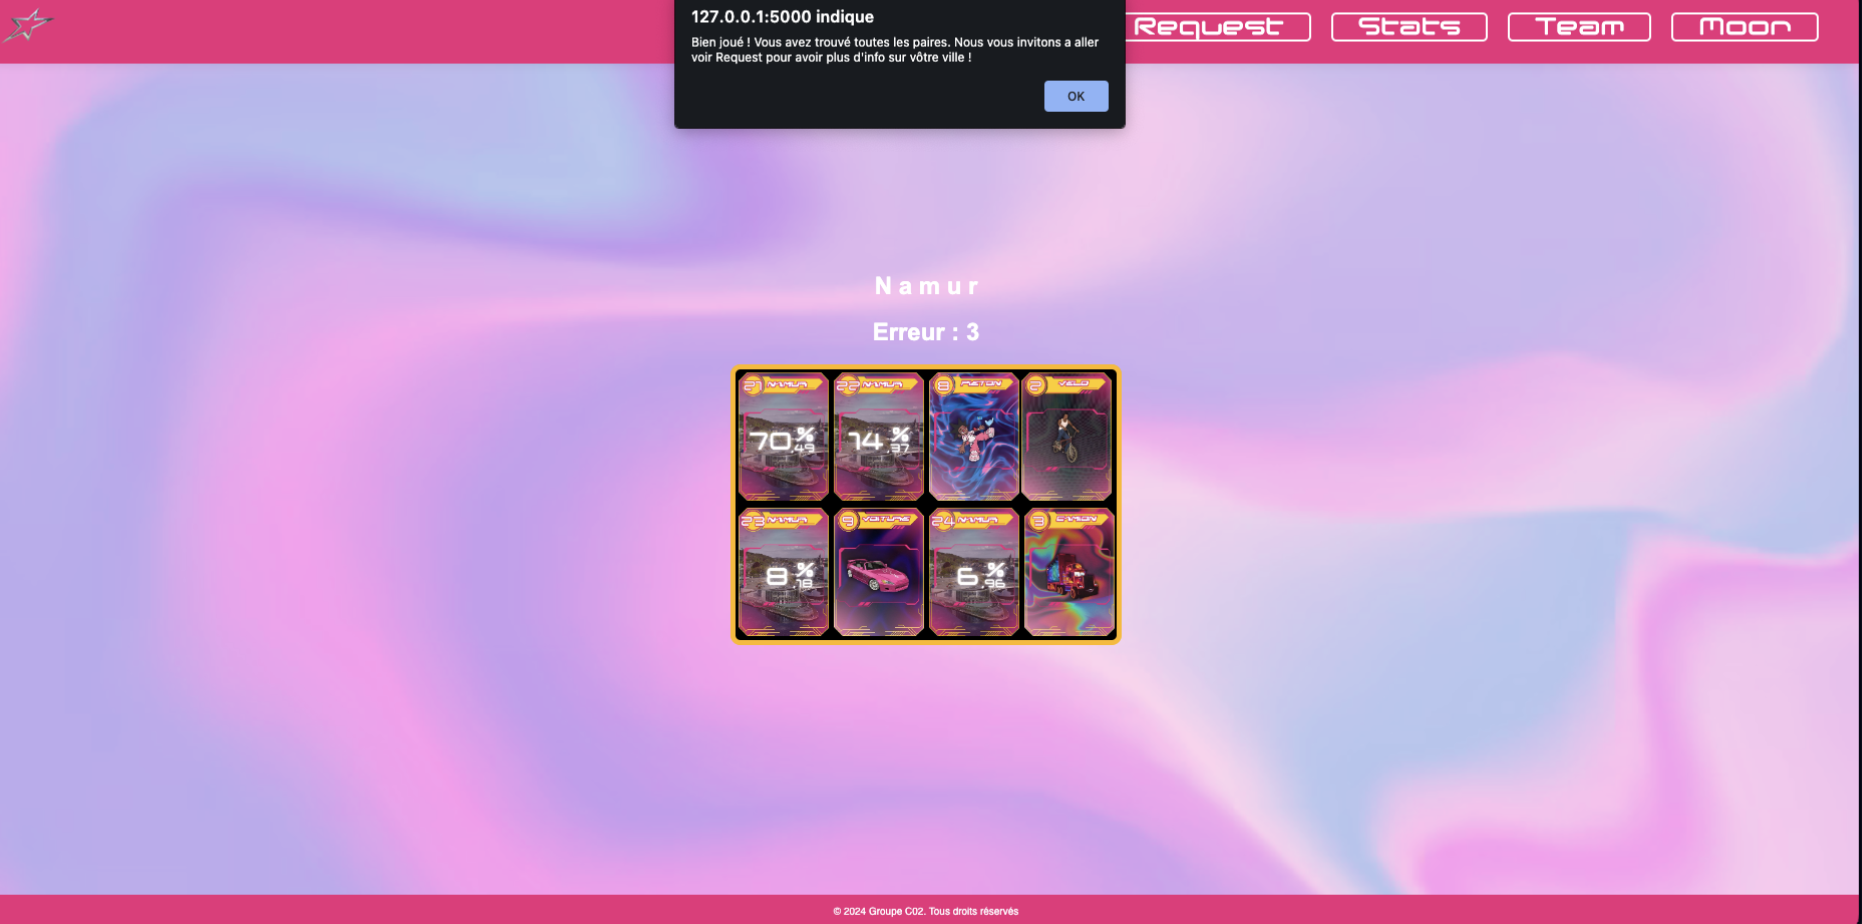
\includegraphics[scale=0.4]{logo/game.png}
\end{center}
Et quand vous avez fini de jouer et trouvé toutes les paires, un message d'alerte vous félicite et vous invite à aller voir la page "request" pour plus d'informations.

Comment avons-nous implémenté ceci ? Le code est principalement en JavaScript et prend en argument la ville choisie, chargeant les différentes cartes qui sont associées à une image comme une voiture, un camion, des vélos, etc.


\section{Peer review}

Je vous conseille d'aller lire nos rapports de peer review.

\section{Dynamique de groupe}

Le groupe n'était pas parfait, certaines personnes ont manqué de participation et les deadlines n'ont pas été respectées.

\section{Conclusion}

Ce projet nous a excités, nous avons adoré et nous avons appris plein de choses.





















\end{document}
